% =============================================================================
% main.tex -- Glioma Brain Digital Twin: Beamer Slide Deck
% CAS Mathematical Challenges in Brain Mechanics -- Finse, March 2026
% =============================================================================
%
% Modular structure: comment out \input lines to shorten the talk.
% Full deck: ~60-70 frames (~90 min lecture/tutorial).
% Short talk: keep sections 1-2, 5-6, 8-9 (~20-25 frames, ~45 min).
%
% Build:  make pdf   (or latexmk -pdf main.tex)
% =============================================================================

% =============================================================================
% preamble.tex -- Beamer preamble for Glioma Brain Digital Twin
% CAS Mathematical Challenges in Brain Mechanics -- Finse, March 2026
% =============================================================================

\documentclass[aspectratio=169,11pt]{beamer}

% --- Theme ---
\usetheme{metropolis}
\metroset{
  progressbar=frametitle,
  numbering=fraction,
  block=fill,
  sectionpage=progressbar
}

% --- Fonts and encoding ---
\usepackage[T1]{fontenc}
\usepackage[utf8]{inputenc}
\usepackage{lmodern}

% --- Math ---
\usepackage{amsmath,amssymb,bm}

% --- Tables ---
\usepackage{booktabs}
\usepackage{tabularx}

% --- Graphics ---
\usepackage{graphicx}
\graphicspath{{figures/}{gslides/}}
\usepackage{tikz}
\usetikzlibrary{arrows.meta, positioning, shapes.geometric, fit, calc}

% --- Code listings (for pipeline commands) ---
\usepackage{listings}
\lstset{
  basicstyle=\ttfamily\scriptsize,
  backgroundcolor=\color{mDarkTeal!5},
  frame=none,
  breaklines=true,
  columns=flexible,
}

% --- Hyperlinks ---
\usepackage{hyperref}

% --- Bibliography ---
\usepackage[backend=biber,style=numeric-comp,maxnames=2,sorting=none]{biblatex}
\addbibresource{references.bib}
\setbeamerfont{footnote}{size=\tiny}

% --- Colors (project-specific) ---
\definecolor{tumorRed}{RGB}{204, 51, 51}
\definecolor{cavityBlue}{RGB}{51, 102, 204}
\definecolor{wmGreen}{RGB}{51, 153, 102}
\definecolor{gmOrange}{RGB}{230, 138, 0}

% --- Bold vector notation macros ---
\newcommand{\bfu}{\bm{u}}
\newcommand{\bfv}{\bm{v}}
\newcommand{\bfx}{\bm{x}}
\newcommand{\bfF}{\bm{F}}
\newcommand{\bfP}{\bm{P}}
\newcommand{\bfC}{\bm{C}}
\newcommand{\bfI}{\bm{I}}
\newcommand{\bfsigma}{\bm{\sigma}}
\newcommand{\bftheta}{\bm{\theta}}
\newcommand{\bfn}{\bm{n}}
\newcommand{\bfb}{\bm{b}}
\newcommand{\bfa}{\bm{a}}
\newcommand{\bfg}{\bm{g}}

% --- Convenience macros ---
\newcommand{\dt}{digital twin}
\newcommand{\DT}{Digital Twin}
\newcommand{\mpmri}{mpMRI}
\newcommand{\credit}[1]{\par\vspace{2pt}{\tiny\textcolor{gray}{#1}}}

% --- Backup slides (don't count in frame numbering) ---
\newcommand{\backupbegin}{%
  \newcounter{framenumberappendix}
  \setcounter{framenumberappendix}{\value{framenumber}}
}
\newcommand{\backupend}{%
  \addtocounter{framenumberappendix}{-\value{framenumber}}
  \addtocounter{framenumber}{\value{framenumberappendix}}
}

% --- Title metadata ---
\title{Glioma Brain Digital Twin}
\subtitle{From Multiparametric MRI to Mathematical Challenges\\
  in Brain Mechanics}
\author{Arvid Lundervold}
\institute{%
  CAS -- Mathematical Challenges in Brain Mechanics\\
  Finse, March 2026}
\date{March 2026}


\begin{document}

% --- Title ---
% =============================================================================
% 01_title.tex -- Title slide
% =============================================================================

{
\setbeamertemplate{footline}{}
\begin{frame}[standout]
  \titlepage
\end{frame}
}


% --- Part I: Context and Motivation ---
% =============================================================================
% 02_motivation.tex -- Introduction and Motivation (~5-6 frames)
% =============================================================================

\section{Motivation}

% ---- Frame 1 ----
\begin{frame}{What Is a Brain Digital Twin?}

  A \alert{Brain Digital Twin} is a subject-specific computational replica
  that can simulate mechanical processes in an individual brain
  \cite{Goriely2015,Meaney2014}.

  \bigskip

  \begin{columns}[T]
    \column{0.55\textwidth}
    \begin{itemize}
      \item Personalized at every layer:
      \begin{itemize}
        \item Geometry from \textbf{this patient's} T1w
        \item Fiber architecture from \textbf{this patient's} dMRI
        \item Functional context from \textbf{this patient's} fMRI
      \end{itemize}
      \item Continuously informed by imaging data
      \item Predicts response to perturbations
    \end{itemize}

    \column{0.4\textwidth}
    % FIGURE SLOT: schematic of digital twin concept
    % \includegraphics[width=\textwidth]{dt_concept_schematic.png}
    \begin{center}
      \fbox{\parbox{0.9\textwidth}{\centering\small
        \textit{Figure:} Digital twin concept\\
        (physical brain $\leftrightarrow$ virtual model)
      }}
    \end{center}
  \end{columns}

\end{frame}

% ---- Frame 2 ----
\begin{frame}{Why Gliomas?}

  Diffuse gliomas present unique challenges for brain mechanics:

  \bigskip

  \begin{itemize}
    \item \textbf{Clinical urgency:} most common primary brain tumors;
      median survival for GBM $\sim$15 months
    \item \textbf{Mass effect:} tumor growth displaces and compresses
      surrounding tissue \cite{Zarodniuk2026}
    \item \textbf{Surgical brain shift:} resection creates cavity,
      CSF dynamics change, tissue deforms
    \item \textbf{Longitudinal changes:} pre-op $\to$ post-op provides
      \emph{empirical deformation data}
    \item \textbf{Pathological anatomy:} standard pipelines break ---
      segmentation, registration, boundary conditions all need adaptation
  \end{itemize}

  \bigskip
  \alert{$\Rightarrow$} Glioma patients are the \emph{hardest} and most
  \emph{clinically relevant} test case for brain digital twins.

\end{frame}

% ---- Frame 3 ----
\begin{frame}{The Finse Workshop Context}

  \textbf{CAS -- Mathematical Challenges in Brain Mechanics}\\
  Finse, March 2026

  \bigskip

  \begin{itemize}
    \item Applied mathematicians $\times$ neuroscientists $\times$
      clinicians
    \item Focus on the \emph{mathematical} difficulties that arise when
      building subject-specific brain models
    \item This talk: a \emph{concrete worked example} grounded in real
      patient data
  \end{itemize}

  \bigskip

  \textbf{Companion project:} Single-subject healthy volunteer
  (\texttt{brain-digital-twin-finse2026})\\
  $\to$ establishes the pipeline; \textbf{this project} extends it to
  pathology and longitudinal change.

\end{frame}

% ---- Frame 4 ----
\begin{frame}{The Governing Equation}

  The mechanical forward problem:
  \[
    \nabla \cdot \bfsigma(\bfu, \bftheta) + \bfb
    = \rho\,\ddot{\bfu}
  \]

  \begin{itemize}
    \item $\bfu(\bfx,t)$ -- displacement field
    \item $\bfsigma$ -- Cauchy stress (from constitutive law)
    \item $\bftheta(\bfx)$ -- spatially varying material parameters
      (stiffness, anisotropy, viscosity)
    \item $\bfb$ -- body forces; $\rho$ -- tissue density
  \end{itemize}

  \bigskip

  MRI informs: the domain $\Omega$ (geometry), the parameter field
  $\bftheta$ (material), and -- partially -- the boundary conditions.

  \bigskip

  \alert{Core difficulty:} non-uniqueness. Many $(\bftheta, \text{BC})$
  combinations explain the same images.

\end{frame}

% ---- Frame 5 ----
\begin{frame}{This Talk: Roadmap}

  \begin{enumerate}
    \item Neuro-oncological challenges
    \item Multiparametric MRI opportunities
    \item Data and metadata (BTC dataset, BIDS)
    \item Processing pipeline (9 steps)
    \item Longitudinal registration and deformation fields
    \item The digital twin concept and architecture
    \item Mathematical challenges
    \item Results preview and outlook
  \end{enumerate}

  \bigskip
  \small
  \textit{Supplemented by Google Slides with Freeview illustrations
  (static and dynamic).}

\end{frame}

% =============================================================================
% 03_neuro_oncology.tex -- Neuro-Oncological Challenges (~5-6 frames)
% =============================================================================

\section{Neuro-Oncological Challenges}

% ---- Frame 1 ----
\begin{frame}{Diffuse Gliomas: Biology and Mechanics}

  \begin{columns}[T]
    \column{0.55\textwidth}
    \begin{itemize}
      \item Infiltrative growth along white matter tracts
      \item Mass effect: compression of adjacent structures
      \item Peritumoral edema: altered tissue properties
      \item Blood-brain barrier disruption
      \item Grades II--IV (WHO 2021 classification)
    \end{itemize}

    \bigskip

    \textbf{Mechanical consequences:}
    \begin{itemize}
      \item Elevated intracranial pressure (ICP)
      \item Midline shift, ventricular compression
      \item Altered viscoelastic properties in tumor zone
    \end{itemize}

    \column{0.4\textwidth}
    % FIGURE SLOT: Freeview T1w with visible tumor (Google Slides)
    \begin{center}
      \fbox{\parbox{0.9\textwidth}{\centering\small
        \textit{GSlides:} T1w showing\\
        glioma mass effect\\[2pt]
        \texttt{FV-01\_t1w\_tumor.png}
      }}
    \end{center}
  \end{columns}

\end{frame}

% ---- Frame 2 ----
\begin{frame}{Surgical Context: Resection and Brain Shift}

  \begin{columns}[T]
    \column{0.55\textwidth}
    \textbf{During surgery:}
    \begin{itemize}
      \item Craniotomy $\to$ CSF drainage $\to$ brain shift
      \item Intraoperative deformation: 10--20\,mm
        \cite{Clatz2005}
      \item Tissue removal creates cavity
    \end{itemize}

    \bigskip

    \textbf{Post-operatively:}
    \begin{itemize}
      \item Resection cavity fills with CSF
      \item Surrounding tissue remodels
      \item Ventricles may expand
      \item Connectivity reorganizes
    \end{itemize}

    \column{0.4\textwidth}
    % FIGURE SLOT: pre-op vs post-op T1w comparison
    \begin{center}
      \fbox{\parbox{0.9\textwidth}{\centering\small
        \textit{GSlides:} Pre-op vs\\
        post-op T1w overlay\\[2pt]
        \texttt{FV-02\_preop\_postop.png}
      }}
    \end{center}
  \end{columns}

  \bigskip

  \alert{Key insight:} The pre-op $\to$ post-op deformation is
  \emph{empirically observable} from MRI --- a rare source of
  ground-truth displacement data for brain mechanics.

\end{frame}

% ---- Frame 3 ----
\begin{frame}{Why Standard Pipelines Fail}

  Pathological anatomy breaks assumptions:

  \bigskip

  \begin{tabular}{lll}
    \toprule
    \textbf{Pipeline step} & \textbf{Assumption} & \textbf{Glioma violation} \\
    \midrule
    FreeSurfer \texttt{recon-all} & Normal cortical folding &
      Tumor displaces cortex \\
    Atlas registration & Diffeomorphic to template &
      Missing tissue (cavity) \\
    Tractography & Coherent WM tracts &
      Infiltrated / disrupted fibers \\
    DTI fitting & Gaussian diffusion &
      Edema alters diffusion \\
    \bottomrule
  \end{tabular}

  \bigskip

  \textbf{Our approach:}
  \begin{itemize}
    \item \texttt{recon-all-clinical} (SynthSeg) for post-op sessions
    \item Automatic resection cavity masking for registration
    \item Cost-function masking in ANTs SyN
  \end{itemize}

\end{frame}

% ---- Frame 4 ----
\begin{frame}{Longitudinal Monitoring: What Changes?}

  Pre-operative $\to$ post-operative comparison reveals:

  \bigskip

  \begin{columns}[T]
    \column{0.48\textwidth}
    \textbf{Structural changes:}
    \begin{itemize}
      \item Resection cavity volume
      \item Ventricular expansion
      \item Cortical thickness alterations
      \item White matter tract disruption
    \end{itemize}

    \column{0.48\textwidth}
    \textbf{Quantifiable via MRI:}
    \begin{itemize}
      \item $\Delta$FA, $\Delta$MD maps (dMRI)
      \item Displacement field $\bfu(\bfx)$ (SyN)
      \item Jacobian $J(\bfx)$ (volume change)
      \item $\Delta$SC, $\Delta$FC matrices
    \end{itemize}
  \end{columns}

  \bigskip

  \alert{$\Rightarrow$} Each quantity has a direct mechanical
  interpretation: displacement, strain, material property change,
  connectivity rewiring.

\end{frame}

% ---- Frame 5 ----
\begin{frame}{Key References}

  \begin{itemize}
    \item \textbf{Aerts et al.\ (2018)} \cite{Aerts2018} --
      Brain dynamics in glioma patients using The Virtual Brain
    \item \textbf{Aerts et al.\ (2022)} \cite{Aerts2022} --
      BTC dataset: pre- and post-operative mpMRI, OpenNeuro ds002080
    \item \textbf{Zarodniuk et al.\ (2026)} \cite{Zarodniuk2026} --
      Mechanical compression induces neuronal apoptosis
    \item \textbf{Clatz et al.\ (2005)} \cite{Clatz2005} --
      Nonrigid registration for intraoperative brain shift
    \item \textbf{Miga et al.\ (2016)} \cite{Miga2016} --
      Model-updated image guidance for brain shift compensation
  \end{itemize}

\end{frame}

% =============================================================================
% 04_mpmri_opportunities.tex -- mpMRI Opportunities (~5-6 frames)
% =============================================================================

\section{Multiparametric MRI Opportunities}

% ---- Frame 1 ----
\begin{frame}{Three Modalities, Three Layers}

  \begin{center}
  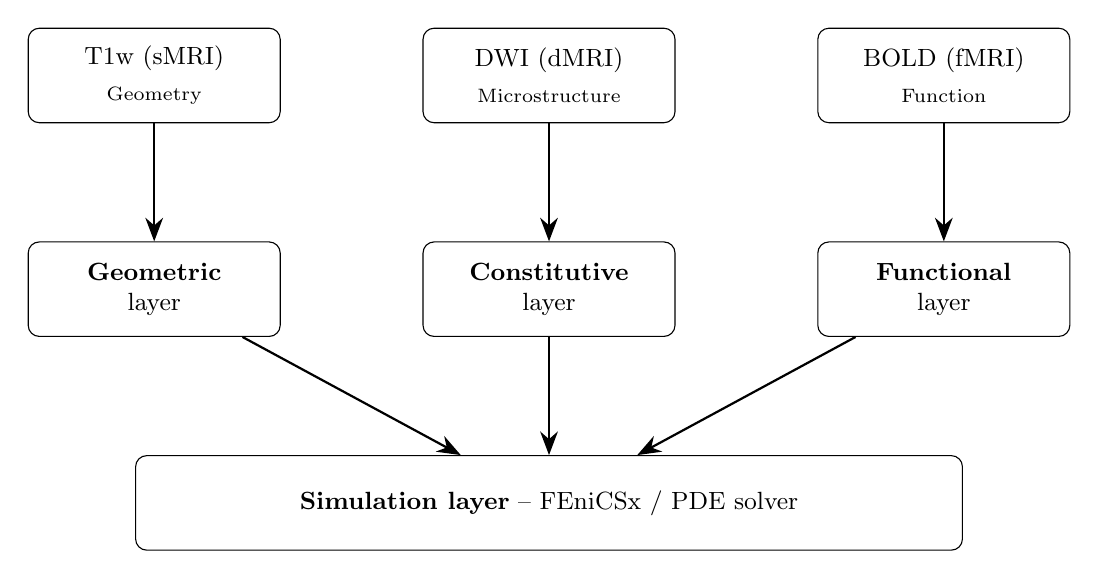
\begin{tikzpicture}[
    box/.style={draw, rounded corners, minimum width=3.2cm,
                minimum height=1.2cm, align=center, font=\small},
    arr/.style={-{Stealth[length=3mm]}, thick},
    node distance=1.8cm
  ]
    \node[box] (smri) {T1w (sMRI)\\[2pt]\scriptsize Geometry};
    \node[box, right=of smri] (dmri) {DWI (dMRI)\\[2pt]\scriptsize Microstructure};
    \node[box, right=of dmri] (fmri) {BOLD (fMRI)\\[2pt]\scriptsize Function};

    \node[box, below=1.5cm of smri] (geo) {\textbf{Geometric}\\layer};
    \node[box, below=1.5cm of dmri] (con) {\textbf{Constitutive}\\layer};
    \node[box, below=1.5cm of fmri] (fun) {\textbf{Functional}\\layer};

    \draw[arr] (smri) -- (geo);
    \draw[arr] (dmri) -- (con);
    \draw[arr] (fmri) -- (fun);

    \node[box, below=1.5cm of con, minimum width=10.5cm]
      (sim) {\textbf{Simulation layer} -- FEniCSx / PDE solver};

    \draw[arr] (geo) -- (sim);
    \draw[arr] (con) -- (sim);
    \draw[arr] (fun) -- (sim);
  \end{tikzpicture}
  \end{center}

\end{frame}

% ---- Frame 2 ----
\begin{frame}{T1w Structural MRI: Geometry}

  \begin{columns}[T]
    \column{0.55\textwidth}
    \begin{itemize}
      \item $1\,\text{mm}$ isotropic MPRAGE
      \item FreeSurfer segmentation:
      \begin{itemize}
        \item Cortical parcellation (Desikan--Killiany)
        \item Subcortical structures (aseg)
        \item Hippocampal subfields, brainstem, thalamic nuclei
      \end{itemize}
      \item Pial and white matter surfaces
      \item Cortical thickness maps
      \item $\to$ FE mesh domain $\Omega$
    \end{itemize}

    \column{0.4\textwidth}
    % FIGURE SLOT: Freeview aparc+aseg overlay
    \begin{center}
      \fbox{\parbox{0.9\textwidth}{\centering\small
        \textit{GSlides:} FreeSurfer\\
        \texttt{aparc+aseg} overlay\\[2pt]
        \texttt{FV-03\_aparc\_aseg.png}
      }}
    \end{center}
  \end{columns}

\end{frame}

% ---- Frame 3 ----
\begin{frame}{Diffusion MRI: Microstructure and Constitutive Properties}

  \begin{columns}[T]
    \column{0.55\textwidth}
    \begin{itemize}
      \item Multi-shell EPI (b = 0, 1000, 2000, 3000\,s/mm$^2$)
      \item AP + PA acquisitions $\to$ distortion correction
      \item DTI fitting: FA, MD, AD, RD maps
      \item Constrained spherical deconvolution (CSD) $\to$ fODFs
      \item Tractography + SIFT2 $\to$ structural connectome
    \end{itemize}

    \bigskip

    \textbf{Mechanical relevance:}\\
    Fiber direction $\bfa_0(\bfx)$ from fODF peaks\\
    Anisotropy ratio from FA\\
    $\to$ transversely isotropic constitutive law

    \column{0.4\textwidth}
    % FIGURE SLOT: FA map + tractography
    \begin{center}
      \fbox{\parbox{0.9\textwidth}{\centering\small
        \textit{GSlides:} FA map and\\
        tractography overlay\\[2pt]
        \texttt{FV-04\_fa\_tracts.png}
      }}
    \end{center}
  \end{columns}

\end{frame}

% ---- Frame 4 ----
\begin{frame}{Functional MRI: Connectivity and Hemodynamics}

  \begin{columns}[T]
    \column{0.55\textwidth}
    \begin{itemize}
      \item Resting-state BOLD EPI
      \item fMRIPrep: motion correction, confound regression,
        SyN-based susceptibility distortion correction
      \item Functional connectivity (FC) matrix
      \item Physiological noise components (cardiac, respiratory)
    \end{itemize}

    \bigskip

    \textbf{Mechanical relevance:}\\
    FC provides spatial priors and zoning\\
    Physiological regressors $\to$ candidate BC drivers\\
    SC--FC coupling $\to$ structure--function relationship

    \column{0.4\textwidth}
    % FIGURE SLOT: FC matrix or BOLD time series
    \begin{center}
      \fbox{\parbox{0.9\textwidth}{\centering\small
        \textit{GSlides:} BOLD signal\\
        and FC matrix\\[2pt]
        \texttt{FV-05\_bold\_fc.png}
      }}
    \end{center}
  \end{columns}

\end{frame}

% ---- Frame 5 ----
\begin{frame}{From mpMRI to Digital Twin: The Pipeline}

  % FIGURE SLOT: workflow diagram (full pipeline)
  \begin{center}
    \fbox{\parbox{0.85\textwidth}{\centering\small
      \textit{Figure:} Full pipeline workflow diagram\\
      T1w/DWI/BOLD $\to$ FreeSurfer/fMRIPrep/QSIPrep/MRtrix3
      $\to$ co-registration $\to$ SC/FC/rsHRF $\to$ mesh $\to$ FE model\\[4pt]
      \texttt{figures/pipeline\_workflow.pdf}\\[4pt]
      \textit{(or TikZ diagram -- see Section 6 for details)}
    }}
  \end{center}

  \bigskip

  Each modality contributes a different \emph{layer} of the digital
  twin. The fully self-contained pipeline transforms raw BIDS NIfTI
  data into co-registered derivatives, connectivity matrices, and
  voxel-wise HRF parameters -- all in native T1w space.

\end{frame}


% --- Part II: Data and Processing ---
% =============================================================================
% 05_data_and_metadata.tex -- Data and Metadata (~4-5 frames)
% =============================================================================

\section{Data and Metadata}

% ---- Frame 1 ----
\begin{frame}{The BTC Dataset (OpenNeuro ds002080)}

  \textbf{Brain Tumor Connectomics} -- Aerts et al.\
  \cite{Aerts2018,Aerts2022}

  \bigskip

  \begin{itemize}
    \item 25 glioma patients, pre- and post-operative mpMRI
    \item T1w, multi-shell DWI, resting-state BOLD per session
    \item We use \textbf{1 subject} $\times$ \textbf{2 timepoints}:
  \end{itemize}

  \bigskip

  \begin{tabular}{llll}
    \toprule
    \textbf{Subject} & \textbf{Session} & \textbf{Tumor} & \textbf{Modalities} \\
    \midrule
    PAT16 & pre-op  & LGG, left hemisphere & T1w, DWI (AP+PA), BOLD \\
    PAT16 & post-op &  (resected)          & T1w, DWI (AP+PA), BOLD \\
    \bottomrule
  \end{tabular}

  \medskip

  \textbf{Phenotypic data} (per session):
  psychosocial questionnaires (STAI, PSWQ, ERQ),
  CANTAB cognitive battery (MOT, RTI, RVP, SOC, SSP)
  $\to$ pre-/post-op \alert{cognitive outcome} tracking.

\end{frame}

% ---- Frame 2 ----
\begin{frame}[fragile]{BIDS Organization}

  Data organized according to the \textbf{Brain Imaging Data Structure}:

  \bigskip

  \begin{columns}[T]
    \column{0.5\textwidth}
    \begin{lstlisting}
data/BIDS_preop_postop/
  participants.tsv
  sub-PAT16/
    sub-PAT16_sessions.tsv
    ses-preop/
      anat/  *_T1w.nii.gz
      dwi/   *_acq-AP_dwi.nii.gz
      func/  *_task-rest_bold...
    ses-postop/
      anat/  ...
      dwi/   ...
      func/  ...
    \end{lstlisting}

    \column{0.45\textwidth}
    \begin{itemize}
      \item Subject $\times$ session hierarchy
      \item AP + PA DWI pairs $\to$ robust distortion correction
      \item JSON sidecars with acquisition parameters
      \item \texttt{*\_sessions.tsv}: 48 cols of clinical \& cognitive data
      \item \texttt{download\_data.py} retrieves from OpenNeuro
    \end{itemize}
  \end{columns}

\end{frame}

% ---- Frame 3 ----
\begin{frame}{Acquisition Parameters}

  \begin{tabular}{llll}
    \toprule
    \textbf{Modality} & \textbf{Sequence} & \textbf{Resolution} & \textbf{Key parameters} \\
    \midrule
    T1w  & MPRAGE & 1\,mm iso & $176 \times 256 \times 256$ \\
    DWI  & EPI    & 2.5\,mm iso & $b = 700,\, 1000,\, 2000$\,s/mm$^2$ \\
    BOLD & EPI    & 3\,mm iso & TR $= 1.7$\,s, resting state \\
    \bottomrule
  \end{tabular}

  \bigskip

  \textbf{Key differences from the healthy-volunteer project:}
  \begin{itemize}
    \item Multi-shell DWI (3 shells vs.\ 4 in healthy)
    \item AP + PA DWI pairs available $\to$ topup-based SDC
    \item Pathological anatomy in all sessions
    \item Two timepoints per subject $\to$ longitudinal analysis
  \end{itemize}

\end{frame}

% ---- Frame 4 ----
\begin{frame}{What the Data Gives Us for Brain Mechanics}

  \begin{center}
  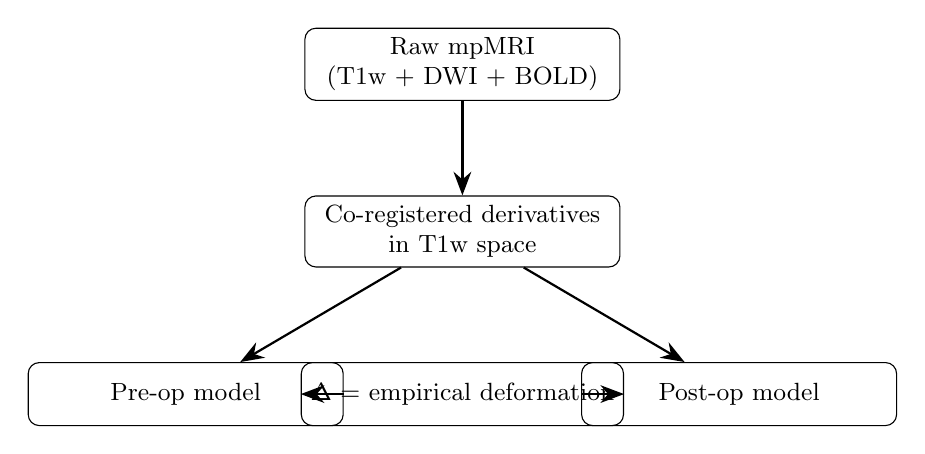
\begin{tikzpicture}[
    box/.style={draw, rounded corners, minimum width=4cm,
                minimum height=0.8cm, align=center, font=\small},
    arr/.style={-{Stealth[length=3mm]}, thick},
    node distance=1.2cm
  ]
    \node[box] (raw) {Raw mpMRI\\(T1w + DWI + BOLD)};
    \node[box, below=of raw] (deriv) {Co-registered derivatives\\in T1w space};
    \node[box, below left=1.2cm and -0.5cm of deriv]
      (pre) {Pre-op model};
    \node[box, below right=1.2cm and -0.5cm of deriv]
      (post) {Post-op model};
    \node[box, below=1.2cm of deriv] (delta) {\alert{$\Delta$ = empirical deformation}};

    \draw[arr] (raw) -- (deriv);
    \draw[arr] (deriv) -- (pre);
    \draw[arr] (deriv) -- (post);
    \draw[arr] (pre) -- (delta);
    \draw[arr] (post) -- (delta);
  \end{tikzpicture}
  \end{center}

  The longitudinal design provides what most brain mechanics studies
  lack: \alert{observed displacement data} for validation.

\end{frame}

% =============================================================================
% 06_processing_pipeline.tex -- Processing Pipeline (~8-10 frames)
% =============================================================================

\section{Processing Pipeline}

% ---- Frame 1 ----
\begin{frame}{Pipeline Overview}

  \begin{center}
  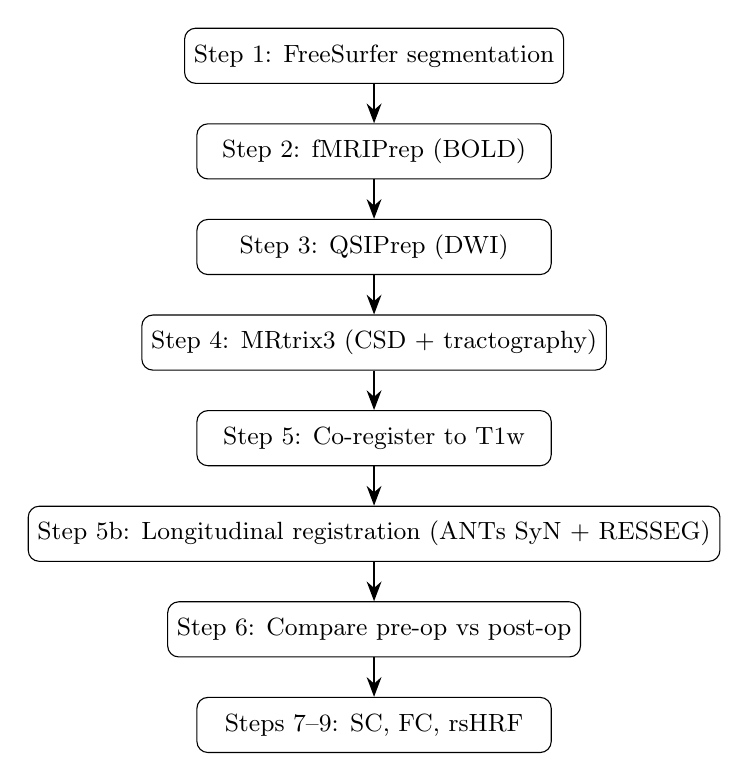
\begin{tikzpicture}[
    pstep/.style={draw, rounded corners, minimum width=4.5cm,
                  minimum height=0.7cm, align=center, font=\small},
    arr/.style={-{Stealth[length=2.5mm]}, thick},
    node distance=0.9cm
  ]
    \node[pstep] (s1) {Step 1: FreeSurfer segmentation};
    \node[pstep, below=0.5cm of s1] (s2) {Step 2: fMRIPrep (BOLD)};
    \node[pstep, below=0.5cm of s2] (s3) {Step 3: QSIPrep (DWI)};
    \node[pstep, below=0.5cm of s3] (s4) {Step 4: MRtrix3 (CSD + tractography)};
    \node[pstep, below=0.5cm of s4] (s5) {Step 5: Co-register to T1w};
    \node[pstep, below=0.5cm of s5] (s5b) {\alert{Step 5b: Longitudinal registration (ANTs SyN + RESSEG)}};
    \node[pstep, below=0.5cm of s5b] (s6) {Step 6: Compare pre-op vs post-op};
    \node[pstep, below=0.5cm of s6] (s79) {Steps 7--9: SC, FC, rsHRF};

    \draw[arr] (s1) -- (s2);
    \draw[arr] (s2) -- (s3);
    \draw[arr] (s3) -- (s4);
    \draw[arr] (s4) -- (s5);
    \draw[arr] (s5) -- (s5b);
    \draw[arr] (s5b) -- (s6);
    \draw[arr] (s6) -- (s79);
  \end{tikzpicture}
  \end{center}

  \small
  Steps 1--5 run per subject $\times$ session.
  Steps 5b--9 are cross-session / per-subject.\\
  \textbf{Self-contained:} only raw BIDS NIfTI + tumor mask required.\\
  Orchestrated by \texttt{run\_pipeline.sh}.

\end{frame}

% ---- Frame 2 ----
\begin{frame}[fragile]{Step 1: FreeSurfer Segmentation}

  \begin{columns}[T]
    \column{0.55\textwidth}
    \begin{itemize}
      \item FreeSurfer 8.1.0 \cite{Fischl2012}
      \item \textbf{Pre-op:} standard \texttt{recon-all}
      \item \textbf{Post-op:} \texttt{recon-all-clinical}\\
        (SynthSeg -- robust to pathology)
      \item Outputs: \texttt{aparc+aseg}, surfaces, cortical thickness
      \item Additional: hippocampal subfields, thalamic nuclei, brainstem
    \end{itemize}

    \bigskip

    \begin{lstlisting}
bash scripts/run_freesurfer.sh \
  --subject PAT16 --session preop
    \end{lstlisting}

    \column{0.4\textwidth}
    % FIGURE SLOT: Freeview recon-all output
    \begin{center}
      \fbox{\parbox{0.9\textwidth}{\centering\small
        \textit{GSlides:} FreeSurfer\\
        segmentation QC\\[2pt]
        \texttt{FV-06\_freesurfer.png}
      }}
    \end{center}
  \end{columns}

\end{frame}

% ---- Frame 3 ----
\begin{frame}{Step 2: fMRIPrep -- BOLD Preprocessing}

  \begin{columns}[T]
    \column{0.55\textwidth}
    \begin{itemize}
      \item fMRIPrep 25.x \cite{Esteban2019}
      \item Skull stripping, motion correction
      \item BOLD-to-T1w boundary-based registration (BBR)
      \item SyN-based susceptibility distortion correction
        (single-PE BOLD)
      \item Confound regression (aCompCor, motion params)
      \item Output: preprocessed BOLD in T1w space
    \end{itemize}

    \column{0.4\textwidth}
    % FIGURE SLOT: fMRIPrep report screenshot
    \begin{center}
      \fbox{\parbox{0.9\textwidth}{\centering\small
        \textit{GSlides:} fMRIPrep\\
        SDC + registration QC\\[2pt]
        \texttt{FV-07\_fmriprep.png}
      }}
    \end{center}
  \end{columns}

\end{frame}

% ---- Frame 4 ----
\begin{frame}{Step 3: QSIPrep -- DWI Preprocessing}

  \begin{columns}[T]
    \column{0.55\textwidth}
    \begin{itemize}
      \item QSIPrep 1.x \cite{Cieslak2021}
      \item AP + PA pairs $\to$ \texttt{topup} for SDC
      \item Eddy current correction, motion correction
      \item Head motion QC (framewise displacement)
      \item Output: corrected DWI, bval/bvec in T1w space
    \end{itemize}

    \bigskip

    \textbf{Advantage over healthy-volunteer project:}\\
    Reverse-PE pairs enable more robust distortion correction
    than fieldmap-less SyN.

    \column{0.4\textwidth}
    % FIGURE SLOT: QSIPrep output / DWI before-after SDC
    \begin{center}
      \fbox{\parbox{0.9\textwidth}{\centering\small
        \textit{GSlides:} QSIPrep\\
        distortion correction\\[2pt]
        \texttt{FV-08\_qsiprep.png}
      }}
    \end{center}
  \end{columns}

\end{frame}

% ---- Frame 5 ----
\begin{frame}{Step 4: MRtrix3 Reconstruction}

  \begin{columns}[T]
    \column{0.55\textwidth}
    \begin{itemize}
      \item MRtrix3 3.x \cite{Tournier2019}
      \item Response function estimation (\texttt{dhollander})
      \item Multi-shell multi-tissue CSD $\to$ fODFs
      \item DTI fitting: FA, MD, AD, RD
      \item Anatomically constrained tractography (ACT)
      \item SIFT2 weighting $\to$ biologically plausible
        connectome
      \item \texttt{tck2connectome} $\to$ structural
        connectivity matrix
    \end{itemize}

    \column{0.4\textwidth}
    % FIGURE SLOT: tractography / fODF glyphs
    \begin{center}
      \fbox{\parbox{0.9\textwidth}{\centering\small
        \textit{GSlides:} Tractography\\
        and fODF glyphs\\[2pt]
        \texttt{FV-09\_tractography.png}
      }}
    \end{center}
  \end{columns}

\end{frame}

% ---- Frame 6 ----
\begin{frame}{Step 5: Co-Registration to T1w Space}

  All derivatives registered to native T1w geometry:

  \bigskip

  \begin{tabular}{llll}
    \toprule
    \textbf{Source} & \textbf{Transform} & \textbf{Tool} & \textbf{Notes} \\
    \midrule
    FreeSurfer $\to$ T1w & Identity / \texttt{mri\_convert} &
      FreeSurfer & Native space \\
    BOLD $\to$ T1w & BBR (from fMRIPrep) &
      fMRIPrep & 6-DOF rigid \\
    DWI $\to$ T1w & FLIRT & FSL & 6-DOF rigid \\
    FA/MD $\to$ T1w & Same as DWI & FSL + MRtrix3 & \\
    fODFs $\to$ T1w & Affine + SH reorient &
      MRtrix3 & Preserves SH basis \\
    Tractogram $\to$ T1w & \texttt{tcktransform} &
      MRtrix3 & Streamline coords \\
    \bottomrule
  \end{tabular}

  \bigskip

  T1w is the untouched reference -- all other modalities are
  resampled \emph{to} it, never the other way around.

\end{frame}

% ---- Frame 7 ----
\begin{frame}[fragile]{Pipeline Orchestration}

  \begin{lstlisting}
bash scripts/run_pipeline.sh \
  --subjects PAT16 \
  --sessions preop,postop \
  --clinical-postop \
  --nthreads 8
  \end{lstlisting}

  \bigskip

  \begin{itemize}
    \item Runs Steps 1--5 for each (subject, session) pair
    \item \texttt{--clinical-postop}: auto-select
      \texttt{recon-all-clinical} for post-op sessions
    \item \texttt{--skip-*} flags to resume from any step
    \item Steps 5b--9 run per-subject after all sessions complete
    \item \texttt{--resseg}: deep-learning cavity masking
      (method-aware cache invalidation)
  \end{itemize}

\end{frame}

% ---- Frame 8 ----
\begin{frame}{Steps 7--9: Connectivity and rsHRF}

  \begin{tabular}{llp{5cm}}
    \toprule
    \textbf{Step} & \textbf{Script} & \textbf{Output} \\
    \midrule
    7. SC & \texttt{compute\_tvb\_connectome.py} &
      $83\times83$ Desikan-Killiany structural connectivity matrix
      (SIFT2-weighted; TVB-ready) \\
    8. FC & \texttt{compute\_fc.py} &
      FC matrix (Pearson + Fisher-$z$), ROI time series,
      confound-regressed \& bandpass-filtered \\
    9. rsHRF & \texttt{compute\_rshrf.py} &
      Voxel-wise FWHM, Height, Time2peak maps
      (point-process deconvolution) \\
    \bottomrule
  \end{tabular}

  \bigskip

  \begin{itemize}
    \item All three steps use pipeline-internal scripts --
      no external tools beyond the core environment
    \item rsHRF replaces the external \texttt{rsHRF} BIDS App
      (unmaintainable \texttt{pyyawt} dependency)
    \item Outputs in \texttt{derivatives/connectivity/} and
      \texttt{derivatives/rshrf/}
  \end{itemize}

\end{frame}

% =============================================================================
% 07_longitudinal_registration.tex -- Longitudinal Registration (~6-8 frames)
% =============================================================================

\section{Longitudinal Registration}

% ---- Frame 1 ----
\begin{frame}{The Longitudinal Registration Problem}

  \textbf{Goal:} Align pre-op and post-op T1w volumes to quantify
  tissue displacement between sessions.

  \bigskip

  \textbf{Why it matters for brain mechanics:}
  \begin{itemize}
    \item The warp field $\bfu(\bfx)$ from diffeomorphic registration
      approximates the \emph{empirical tissue displacement}
    \item Jacobian $J(\bfx) = \det(\bfI + \nabla\bfu)$ encodes
      \emph{local volume change}
    \item These provide rare \alert{validation data} for FE model
      predictions
  \end{itemize}

  \bigskip

  \textbf{Challenge:} The resection cavity is a topological change ---
  tissue that existed pre-op is gone post-op. Standard registration
  tries to ``explain'' the cavity, producing artifacts.

\end{frame}

% ---- Frame 2 ----
\begin{frame}{The Cavity Masking Problem}

  \begin{columns}[T]
    \column{0.5\textwidth}
    \textbf{Without masking:}
    \begin{itemize}
      \item SyN tries to deform healthy tissue into the surgical void
      \item Produces unrealistic deformation near cavity
      \item Contaminates displacement and Jacobian maps
    \end{itemize}

    \bigskip

    \textbf{With masking:}
    \begin{itemize}
      \item Cavity region excluded from cost function
      \item SyN optimizes only on intact tissue
      \item Biologically plausible deformation field
    \end{itemize}

    \column{0.45\textwidth}
    % FIGURE SLOT: cavity mask overlay
    \begin{center}
      \fbox{\parbox{0.9\textwidth}{\centering\small
        \textit{GSlides:} Cavity mask\\
        overlay on post-op T1w\\[2pt]
        \texttt{FV-10\_cavity\_mask.png}
      }}
    \end{center}
  \end{columns}

\end{frame}

% ---- Frame 3 ----
\begin{frame}{Automatic Cavity Detection: Three Tiers}

  \textbf{Tier 1 (default):} Tumor-mask prior
  \begin{itemize}
    \item Resample the pre-op tumor mask into post-op T1w space
    \item Threshold at $p > 0.5$ $\to$ binary cavity seed
    \item Reliable when a pre-op tumor mask exists
  \end{itemize}

  \medskip

  \textbf{Tier 2 (fallback):} SynthSeg segmentation difference
  \begin{itemize}
    \item Compare pre-op and post-op \texttt{aparc+aseg}: brain $\to$
      CSF = cavity
    \item Sensitive to grid-size and label-convention mismatches
  \end{itemize}

  \medskip

  \textbf{Tier 3 (optional):} RESSEG deep learning model
  \cite{PerezGarcia2021}
  \begin{itemize}
    \item Enabled via \texttt{--resseg} flag
    \item Trained for postoperative cavity segmentation, but may
      mislocalize on atypical anatomies
  \end{itemize}

  \medskip

  All tiers produce a binary mask $\to$ inverted for ANTs \texttt{-x}
  flag (1 = healthy, 0 = cavity).
  Method-aware caching: switching tier auto-clears the mask
  \emph{and} all downstream outputs.

\end{frame}

% ---- Frame 3b: Diagnostic case study ----
\begin{frame}{Case Study: When Cavity Masking Fails}

  On sub-PAT16, RESSEG (Tier~3) produced a mask \alert{$\sim$50\,mm from
  the actual resection cavity}:

  \medskip

  \begin{tabular}{lrr}
    \toprule
    \textbf{Mask} & \textbf{Centre of mass (mm)} & \textbf{Volume} \\
    \midrule
    Pre-op tumor (Aerts) & $(30,\; 37,\; {-}13)$ & 45.4\,cm$^3$ \\
    RESSEG cavity        & $(53,\; {-}5,\; {-}21)$ & 18.6\,cm$^3$ \\
    Tumor-prior (Tier~1) & $(31,\; 36,\; {-}13)$ & 45.2\,cm$^3$ \\
    \bottomrule
  \end{tabular}

  \medskip

  \textbf{Consequence cascade:}
  \begin{itemize}
    \item Overlap between RESSEG mask and warped tumor: \alert{0\%}
    \item SyN excluded normal tissue, tried to match the actual cavity
    \item Global T1w correlation: \alert{0.66} (expected $> 0.85$)
    \item All 21 longitudinal outputs unreliable
  \end{itemize}

  \medskip

  \alert{Lesson:} Empirical verification of cavity masks is essential
  before downstream mechanics analysis.

\end{frame}

% ---- Frame 4 ----
\begin{frame}[fragile]{ANTs SyN with Cost Function Masking}

  \begin{lstlisting}
antsRegistrationSyN.sh \
  -d 3 \
  -f postop_T1w.nii.gz \     # fixed (post-op)
  -m preop_T1w.nii.gz  \     # moving (pre-op)
  -x cavity_mask_inv.nii.gz \ # cost function mask
  -t s \                      # SyN transform
  -n 8                        # threads
  \end{lstlisting}

  \bigskip

  \textbf{ANTs SyN} \cite{Avants2008}: symmetric diffeomorphic
  registration with cross-correlation.

  \bigskip

  \textbf{Outputs:}
  \begin{itemize}
    \item Forward warp: $\bfu(\bfx)$ (pre-op $\to$ post-op)
    \item Inverse warp: $\bfu^{-1}(\bfx)$ (post-op $\to$ pre-op)
    \item Affine component: initial linear alignment
  \end{itemize}

\end{frame}

% ---- Frame 5 ----
\begin{frame}{Deformation Field Outputs}

  From the SyN warp field we compute:

  \bigskip

  \begin{tabular}{lll}
    \toprule
    \textbf{Output} & \textbf{Definition} & \textbf{Interpretation} \\
    \midrule
    Displacement $|\bfu(\bfx)|$ &
      $\sqrt{u_1^2 + u_2^2 + u_3^2}$ &
      Tissue motion (mm) \\[4pt]
    Jacobian $J(\bfx)$ &
      $\det(\bfI + \nabla\bfu)$ &
      $J > 1$: expansion \\
    & & $J < 1$: contraction \\[4pt]
    Cavity mask & Binary &
      Resection void \\
    \bottomrule
  \end{tabular}

  \bigskip

  \begin{itemize}
    \item Displacement: where did tissue move, and how far?
    \item Jacobian: which regions expanded (e.g., ventricles) or
      contracted (e.g., near resection)?
    \item ROI-level statistics: mean displacement and Jacobian
      per brain region
  \end{itemize}

\end{frame}

% ---- Frame 6 ----
\begin{frame}{Warping Pre-op Derivatives to Post-op Space}

  With the SyN warp, we can bring \emph{any} pre-op derivative into
  post-op space for consistent voxel-wise comparison:

  \bigskip

  \begin{itemize}
    \item T1w (linear interpolation)
    \item FA, MD, AD, RD maps (linear interpolation)
    \item \texttt{aparc+aseg} (nearest-neighbor interpolation)
  \end{itemize}

  \bigskip

  \textbf{Result:} $\Delta\text{FA}(\bfx) = \text{FA}_{\text{post}}(\bfx)
  - \text{FA}_{\text{pre}\to\text{post}}(\bfx)$ is now a geometrically
  correct voxel-wise comparison, not contaminated by brain shift.

  \bigskip

  % FIGURE SLOT: warped pre-op T1w vs post-op T1w (checkerboard)
  \begin{center}
    \fbox{\parbox{0.7\textwidth}{\centering\small
      \textit{GSlides:} Warped pre-op T1w aligned with post-op T1w\\
      + displacement magnitude overlay\\[2pt]
      \texttt{FV-11\_warped\_alignment.png}
    }}
  \end{center}

\end{frame}

% ---- Frame 7 ----
\begin{frame}{Brain Mechanics Relevance of Deformation Fields}

  \begin{itemize}
    \item \textbf{Displacement field} $\bfu(\bfx)$: empirical tissue
      motion between pre-op and post-op
      \begin{itemize}
        \item Validation target for FE model predictions
        \item Spatial pattern reveals deformation mode
          (compression, shear, rotation)
      \end{itemize}
    \item \textbf{Jacobian} $J(\bfx)$: local volume change
      \begin{itemize}
        \item $J > 1$ near ventricles $\Rightarrow$ post-op expansion
        \item $J < 1$ near resection $\Rightarrow$ tissue collapse
        \item Regions where $J \neq 1$ require large-deformation
          formulations
      \end{itemize}
    \item \textbf{Cavity mask}: defines a new boundary condition surface
      for the post-op FE model
  \end{itemize}

  \bigskip

  \alert{These outputs bridge imaging and mechanics:}\\
  registration $\to$ displacement $\to$ strain $\to$ stress
  (via constitutive law).

\end{frame}


% --- Part III: Modeling and Mathematics ---
% =============================================================================
% 08_digital_twin_concept.tex -- Digital Twin Architecture (~6-8 frames)
% =============================================================================

\section{The Digital Twin Concept}

% ---- Frame 1 ----
\begin{frame}{Five-Layer Architecture}

  \begin{center}
  \begin{tikzpicture}[
    layer/.style={draw, rounded corners, minimum width=10cm,
                  minimum height=0.9cm, align=center, font=\small},
    arr/.style={-{Stealth[length=2.5mm]}, thick},
    node distance=0.5cm
  ]
    \node[layer] (L1) {\textbf{Layer 1: Geometric} --
      patient-specific FE mesh from T1w segmentation};
    \node[layer, below=of L1] (L2) {\textbf{Layer 2: Constitutive} --
      heterogeneous, anisotropic material properties from dMRI};
    \node[layer, below=of L2] (L3) {\textbf{Layer 3: Functional} --
      connectivity patterns and hemodynamic priors from fMRI};
    \node[layer, below=of L3] (L4) {\textbf{Layer 4: Simulation} --
      PDE solver (FEniCSx): displacement, stress, strain};
    \node[layer, below=of L4, fill=structure!15] (L5)
      {\textbf{Layer 5: Clinical Outcome} --
      cognitive \& psychosocial assessment (CANTAB, questionnaires)};

    \draw[arr] (L1) -- (L2);
    \draw[arr] (L2) -- (L3);
    \draw[arr] (L3) -- (L4);
    \draw[arr] (L4) -- (L5);
    \draw[arr, dashed, bend left=40] (L5.east) to
      node[right, font=\scriptsize, align=left]
        {validation\\feedback} (L4.east);
  \end{tikzpicture}
  \end{center}

  Each layer is \emph{personalized}: geometry from this patient's T1w,
  fibers from this patient's dMRI, function from this patient's fMRI,
  and outcomes from this patient's cognitive battery.

\end{frame}

% ---- Frame 2 ----
\begin{frame}{Layer 1: Patient-Specific Geometry}

  \begin{columns}[T]
    \column{0.55\textwidth}
    \begin{itemize}
      \item T1w segmentation $\to$ tissue label map
      \item Marching cubes $\to$ surface extraction
      \item Gmsh \cite{Geuzaine2009} $\to$ tetrahedral volume mesh
      \item Compartment tagging (GM, WM, CSF, deep nuclei, \ldots)
      \item Adaptive element sizing: finer near surfaces
    \end{itemize}

    \bigskip

    \textbf{Glioma-specific:}
    \begin{itemize}
      \item Pre-op mesh includes tumor region
      \item Post-op mesh includes cavity as boundary
      \item Mesh quality at irregular geometry
    \end{itemize}

    \column{0.4\textwidth}
    % FIGURE SLOT: FE mesh visualization
    \begin{center}
      \fbox{\parbox{0.9\textwidth}{\centering\small
        \textit{Figure:} Tetrahedral mesh\\
        with tissue compartments\\[2pt]
        \texttt{figures/fe\_mesh.png}
      }}
    \end{center}
  \end{columns}

\end{frame}

% ---- Frame 3 ----
\begin{frame}{Layer 2: dMRI-Informed Constitutive Properties}

  \textbf{Isotropic tissues} (cortical GM, deep nuclei, hippocampus):
  \[
    W_{\text{iso}} = \frac{\mu}{2}(\bar{I}_1 - 3)
      + \frac{\kappa}{2}(J - 1)^2
    \qquad \text{(neo-Hookean)}
  \]

  \textbf{Anisotropic tissues} (WM, corpus callosum, brainstem):
  \[
    W_{\text{aniso}} = W_{\text{iso}}
      + \frac{k_1}{2k_2}\left[
        \exp\!\bigl(k_2 \langle I_4 - 1 \rangle^2\bigr) - 1
      \right]
  \]
  where $I_4 = \bfa_0 \cdot \bfC\, \bfa_0$, with fiber direction
  $\bfa_0(\bfx)$ from fODF peaks and $k_1 \propto \text{FA}$.

  \bigskip

  \begin{tabular}{lll}
    \toprule
    \textbf{Tissue} & $\mu$ (kPa) & \textbf{Model} \\
    \midrule
    Cortical GM  & 2.0 & Isotropic neo-Hookean \\
    Cerebral WM  & 1.5 & Transversely isotropic (Holzapfel) \\
    Deep nuclei  & 2.5 & Isotropic \\
    CSF          & $10^{-3}$ & Penalty stiffness \\
    \bottomrule
  \end{tabular}

\end{frame}

% ---- Frame 4 ----
\begin{frame}{Layer 3: Functional Connectivity}

  \begin{columns}[T]
    \column{0.48\textwidth}
    \textbf{Structural connectivity (SC):}
    \begin{itemize}
      \item \texttt{compute\_tvb\_connectome.py} (Step 7)
      \item SIFT2-weighted streamline counts
      \item $83\times83$ Desikan-Killiany matrix
    \end{itemize}

    \bigskip

    \textbf{SC--FC coupling:}
    \begin{itemize}
      \item Pearson correlation between SC and FC
      \item Regions of high SC--FC coupling $\to$ well-constrained
      \item Regions of low coupling $\to$ functionally plastic
    \end{itemize}

    \column{0.48\textwidth}
    \textbf{Functional connectivity (FC):}
    \begin{itemize}
      \item \texttt{compute\_fc.py} (Step 8)
      \item Band-pass filtered, confound-regressed, scrubbed
      \item Pearson correlation + Fisher-$z$ transform
    \end{itemize}

    \bigskip

    % FIGURE SLOT: SC and FC matrices side by side
    \begin{center}
      \fbox{\parbox{0.9\textwidth}{\centering\small
        \textit{GSlides:} SC vs FC\\
        matrices (pre-op)\\[2pt]
        \texttt{FV-12\_sc\_fc.png}
      }}
    \end{center}
  \end{columns}

\end{frame}

% ---- Frame 5 ----
\begin{frame}{Layer 4: The Forward Problem}

  Find $\bfu \in V$ such that $\forall\, \bfv \in V_0$:
  \[
    \int_{\Omega_0} \bfP(\bfu) : \nabla_0 \bfv \,\mathrm{d}V
    = \int_{\Omega_0} \rho_0 \,\bfb \cdot \bfv \,\mathrm{d}V
    + \int_{\Gamma_{\text{vent}}} p_{\text{CSF}} \,
      J\,\bfF^{-\mathrm{T}}\bfn_0 \cdot \bfv \,\mathrm{d}A
  \]

  \begin{itemize}
    \item $\bfP = \partial W / \partial \bfF$ -- first Piola--Kirchhoff
      stress
    \item $\bfF = \bfI + \nabla_0\bfu$ -- deformation gradient
    \item Newton iteration via PETSc/SNES through FEniCSx/DOLFINx
      \cite{Baratta2023}
    \item Near-incompressibility: $\kappa = 100\,\mu$
  \end{itemize}

  \bigskip

  \textbf{Boundary conditions:}
  \begin{enumerate}
    \item Gravity (supine) + clamped skull
    \item Gravity (prone vs.\ supine)
    \item Intracranial pressure on ventricular surface
  \end{enumerate}

\end{frame}

% ---- Frame 6 ----
\begin{frame}{Layer 5: Clinical Outcome Validation}

  The mechanical model predicts \emph{where} tissue deforms and
  \emph{which} tracts are disrupted. Layer~5 asks:
  \alert{did this matter for the patient?}

  \bigskip

  \begin{columns}[T]
    \column{0.48\textwidth}
    \textbf{Cognitive battery (CANTAB):}
    \begin{itemize}
      \item MOT -- motor screening
      \item RTI -- reaction time (simple + 5-choice)
      \item RVP -- sustained attention ($A'$)
      \item SOC -- spatial planning (Stockings)
      \item SSP -- spatial working memory span
    \end{itemize}

    \column{0.48\textwidth}
    \textbf{Psychosocial:}
    \begin{itemize}
      \item STAI -- trait anxiety
      \item PSWQ -- worry
      \item ERQ -- emotion regulation
      \item UCLA Loneliness
    \end{itemize}
  \end{columns}

  \bigskip

  \textbf{Closing the loop:}
  \begin{enumerate}
    \item Simulation predicts tract disruption in region $r$
    \item Map $r$ to DK parcels $\to$ identify affected cognitive domain
    \item Compare predicted deficit with observed $\Delta\text{CANTAB}$
    \item Discrepancies $\to$ model refinement (functional plasticity?)
  \end{enumerate}

\end{frame}

% ---- Frame 7 ----
\begin{frame}{Glioma vs.\ Healthy: What Changes in the Twin?}

  \begin{tabular}{lll}
    \toprule
    \textbf{Layer} & \textbf{Healthy} & \textbf{Glioma} \\
    \midrule
    Geometry & Normal anatomy &
      Tumor mass / cavity / shifted anatomy \\
    Constitutive & Standard $\mu$, FA &
      Altered diffusion in infiltration zone \\
    Functional & Normal FC &
      Reorganized connectivity \\
    Boundary & Skull + ventricles &
      + cavity surface (new BC) \\
    Validation & No displacement data &
      \alert{Pre-op $\to$ post-op deformation} \\
    Clinical outcome & No deficit data &
      \alert{CANTAB $\Delta$ pre $\to$ post} \\
    \bottomrule
  \end{tabular}

  \bigskip

  The glioma digital twin is harder to build but offers something
  the healthy twin cannot: \alert{observed mechanical deformation}
  \emph{and} \alert{measured cognitive outcomes} from longitudinal data.

\end{frame}

% =============================================================================
% 09_math_challenges.tex -- Mathematical Challenges (~8-10 frames)
% =============================================================================

\section{Mathematical Challenges}

% ---- Frame 1: Overview ----
\begin{frame}{Seven + One Challenges}

  From the companion concept note, adapted for glioma:

  \bigskip

  \begin{enumerate}
    \item The ill-posed inverse problem
    \item Constitutive modeling from dMRI
    \item Registration error amplification
    \item Boundary conditions and unknown forcing
    \item Multimodal fusion across scales
    \item Uncertainty quantification
    \item Validation without ground truth
    \item[\alert{8.}] \alert{Pathological tissue and post-surgical
      deformation}
  \end{enumerate}

  \bigskip

  Challenges 1--7 apply to any brain digital twin.\\
  Challenge 8 is specific to neuro-oncology.

\end{frame}

% ---- Frame 2 ----
\begin{frame}{Challenge 1: The Ill-Posed Inverse Problem}

  The map from MRI observables to material parameters $\bftheta(\bfx)$
  is \emph{non-unique}.

  \bigskip

  \begin{itemize}
    \item Different $(\bftheta, \text{BC})$ combinations produce similar
      predicted observables
    \item Without direct displacement measurements (MRE, tagged MRI),
      the inverse problem is severely underdetermined
  \end{itemize}

  \bigskip

  \textbf{Research questions:}
  \begin{itemize}
    \item Identifiability of mechanical parameters from
      sMRI + dMRI + fMRI alone?
    \item Can SC + FC provide sufficient constraints?
    \item \alert{Glioma advantage:} longitudinal deformation data
      $\bfu(\bfx)$ from SyN provides additional constraints on
      $\bftheta$
  \end{itemize}

\end{frame}

% ---- Frame 3 ----
\begin{frame}{Challenge 2: Constitutive Modeling from dMRI}

  \begin{columns}[T]
    \column{0.55\textwidth}
    \begin{itemize}
      \item DTI $\to$ mechanics mapping is a \emph{modeling assumption},
        not measured \cite{Giordano2014}
      \item Crossing fibers: DTI principal eigenvector is misleading
      \item Partial volume contamination at boundaries
      \item Exponential fiber stiffening:
    \end{itemize}

    \[
      \psi_f = \frac{k_1}{2k_2}
        \left[\exp(k_2 \langle I_4 - 1\rangle^2) - 1\right]
    \]

    Effect is small at physiological strains ($< 1\%$),\\
    significant at traumatic strains ($> 10\%$).

    \column{0.4\textwidth}
    \alert{Glioma-specific:}
    \begin{itemize}
      \item Tumor infiltration alters diffusion properties
      \item Peritumoral edema: increased MD, decreased FA
      \item How to model the tumor--brain interface?
      \item Constitutive law in the infiltration zone?
    \end{itemize}
  \end{columns}

\end{frame}

% ---- Frame 4 ----
\begin{frame}{Challenge 3: Registration and Error Amplification}

  Mechanics depends on \emph{spatial derivatives} (strain $=$
  gradient of displacement). Differentiation amplifies errors.

  \bigskip

  \begin{itemize}
    \item Registration between modalities is itself ill-posed
    \item Registration warps $\neq$ physical displacements
    \item Diffeomorphic registration can introduce deformations the
      mechanical model misinterprets
  \end{itemize}

  \bigskip

  \textbf{Research questions:}
  \begin{itemize}
    \item How does registration uncertainty propagate to stress/strain?
    \item ``Mechanical registration error'': predicted mechanics from
      plausible alternative registrations?
  \end{itemize}

  \medskip

  \alert{Glioma -- concrete example:} A mislocated cavity mask
  ($\sim$50\,mm off) caused global T1w correlation to drop from
  $> 0.85$ to 0.66, with displacement artifacts of 2.4\,mm at the
  actual cavity.  All downstream mechanics would have been built on
  corrupted deformation fields.

\end{frame}

% ---- Frame 5 ----
\begin{frame}{Challenge 4: Boundary Conditions}

  \begin{columns}[T]
    \column{0.55\textwidth}
    \textbf{Standard BC surfaces:}
    \begin{itemize}
      \item Skull: fixed, sliding, or frictional?
      \item Ventricles: pressure BC or FSI?
      \item Falx / tentorium: rigid membrane?
    \end{itemize}

    \bigskip

    \textbf{Glioma-specific BC:}
    \begin{itemize}
      \item \alert{Resection cavity}: new free surface
      \item Cavity filled with CSF: pressure BC?
      \item Cavity wall: scarred tissue, different properties?
      \item Tumor--brain interface: traction-free or infiltrated?
    \end{itemize}

    \column{0.4\textwidth}
    % FIGURE SLOT: schematic of BC surfaces
    \begin{center}
      \fbox{\parbox{0.9\textwidth}{\centering\small
        \textit{Figure:} Boundary\\
        condition surfaces\\
        (skull, ventricles,\\
        cavity)\\[2pt]
        \texttt{figures/bc\_schematic.pdf}
      }}
    \end{center}
  \end{columns}

\end{frame}

% ---- Frame 6 ----
\begin{frame}{Challenge 5: Multimodal Fusion Across Scales}

  \begin{tabular}{lll}
    \toprule
    \textbf{Modality} & \textbf{Scale} & \textbf{Timescale} \\
    \midrule
    dMRI & Sub-voxel ($\mu$m fibers) & Snapshot \\
    fMRI & Voxel-level hemodynamics & Seconds \\
    Mechanics & Mesh element ($\sim$mm) &
      ms (waves) to months (remodeling) \\
    \bottomrule
  \end{tabular}

  \bigskip

  \textbf{Research questions:}
  \begin{itemize}
    \item Spatial scale mismatch: voxel dMRI $\to$ element FE mesh?
    \item Can fMRI temporal information (pulsatile components)
      inform mechanical BCs despite timescale gap?
    \item Joint assimilation framework for sMRI + dMRI + fMRI into
      a mechanical model?
    \item \alert{Glioma:} tumor heterogeneity adds yet another scale
      (microscopic infiltration $\to$ macroscopic deformation)
  \end{itemize}

\end{frame}

% ---- Frame 7 ----
\begin{frame}{Challenge 6: Uncertainty Quantification}

  A credible digital twin must quantify uncertainty.
  Bayesian inversion:
  \[
    p(\bftheta \mid \mathbf{y})
      \propto p(\mathbf{y} \mid \bftheta)\,p(\bftheta)
  \]
  is attractive but computationally prohibitive with fine 3D meshes.

  \bigskip

  \textbf{Approaches:}
  \begin{itemize}
    \item Region-wise parameterization (reduce dimensionality)
    \item Laplace approximation, variational inference
    \item Surrogate models (polynomial chaos, neural network)
    \item Sensitivity indices (Sobol, adjoint-based)
  \end{itemize}

  \bigskip

  \alert{Glioma:} the tumor infiltration zone introduces additional
  parametric uncertainty. ``How far does the tumor extend?'' is
  itself uncertain, and this uncertainty propagates into the
  mechanical prediction.

\end{frame}

% ---- Frame 8 ----
\begin{frame}{Challenge 7: Validation}

  Without MRE, how do we validate?

  \bigskip

  \begin{itemize}
    \item Falsifiability: does anisotropic $\neq$ isotropic?
    \item Cross-modal consistency: stress $\sim$ FC patterns?
    \item Literature comparison: stiffness vs.\ published MRE values
  \end{itemize}

  \bigskip

  \alert{Glioma advantage} (unique to this project):
  \begin{itemize}
    \item Pre-op $\to$ post-op displacement field from SyN
      provides \emph{observed} deformation
    \item Can the FE model predict the spatial pattern of
      $|\bfu(\bfx)|$ under surgery-like boundary conditions?
    \item Jacobian map: does the model predict correct
      expansion/contraction pattern?
  \end{itemize}

  \medskip

  \textbf{Sensitivity analysis as a feature:} The probabilistic tumor
  mask enables running the simulation at thresholds $p > 0.3$, $0.5$,
  $0.7$ -- quantifying how segmentation uncertainty propagates into
  the predicted displacement field.

  \medskip

  This is the closest to \alert{ground-truth displacement data}
  available from clinical MRI alone.

\end{frame}

% ---- Frame 9 ----
\begin{frame}{Challenge 8: Pathological Tissue (Glioma-Specific)}

  New mathematical difficulties introduced by pathology:

  \bigskip

  \begin{itemize}
    \item \textbf{Tumor infiltration zone:} gradual transition from
      normal to pathological tissue properties --- not a sharp boundary
    \item \textbf{Mass effect modeling:} tumor growth as a volumetric
      source term; reaction-diffusion PDE coupled to mechanics
      \cite{Hormuth2021}
    \item \textbf{Post-surgical remodeling:} time-dependent material
      property changes (scarring, gliosis)
    \item \textbf{Topological change:} pre-op domain $\neq$ post-op
      domain (cavity creation)
    \item \textbf{Data contamination:} diffusion/functional signals in
      peri-tumoral region are pathologically altered, not just noisy
  \end{itemize}

  \bigskip

  These are not just ``more noise'' --- they represent \emph{qualitative}
  changes in the mathematical structure of the problem.

\end{frame}


% --- Part IV: Outlook ---
% =============================================================================
% 10_results_and_outlook.tex -- Results Preview and Outlook (~4-5 frames)
% =============================================================================

\section{Results and Outlook}

% ---- Frame 1 ----
\begin{frame}{Current Status}

  \begin{tabular}{llc}
    \toprule
    \textbf{Component} & \textbf{Description} & \textbf{Status} \\
    \midrule
    Data & BIDS organization (PAT16 $\times$ 2 sessions)\footnote{Full cohort (25 patients) on OpenNeuro ds002080.} &
      \checkmark \\
    Step 1 & FreeSurfer segmentation (+ clinical) &
      \checkmark \\
    Step 2 & fMRIPrep BOLD preprocessing &
      \checkmark \\
    Step 3 & QSIPrep DWI preprocessing &
      \checkmark \\
    Step 4 & MRtrix3 CSD + tractography &
      \checkmark \\
    Step 5 & Co-registration to T1w &
      \checkmark \\
    Step 5b & Longitudinal registration (ANTs SyN) &
      \checkmark\footnote{Re-run with tumor-prior (Tier~1) after
      RESSEG cavity mask was found mislocated by $\sim$50\,mm.} \\
    Step 6 & Pre-op vs post-op comparison &
      \checkmark \\
    Step 7 & Structural connectivity (TVB) &
      \checkmark \\
    Step 8 & Functional connectivity + ROI time series &
      \checkmark \\
    Step 9 & rsHRF estimation (point-process deconv.) &
      \checkmark \\
    \midrule
    FE mesh & Gmsh tetrahedral meshing (192k tets) &
      \checkmark \\
    Materials & DTI-informed constitutive mapping &
      \checkmark \\
    Forward solver & FEniCSx brain shift simulation &
      \checkmark \\
    Mass effect & Tumour rebound body force model &
      \checkmark \\
    Validation & FEM vs.\ ANTs displacement comparison &
      \checkmark \\
    Coupling & FEM $\to$ Hopf neural mass (NB08) &
      \checkmark \\
    \bottomrule
  \end{tabular}

\end{frame}

% ---- Frame 2 ----
\begin{frame}{Preliminary Results: Longitudinal Deformation}

  \begin{columns}[T]
    \column{0.48\textwidth}
    % FIGURE SLOT: displacement magnitude map
    \begin{center}
      \fbox{\parbox{0.95\textwidth}{\centering\small
        \textit{GSlides:} Displacement\\
        magnitude map $|\bfu(\bfx)|$\\[2pt]
        \texttt{FV-13\_displacement.png}
      }}
    \end{center}

    \bigskip

    \begin{itemize}
      \item High displacement near cavity
      \item Ventricular expansion (J $> 1$)
      \item Far-field displacement decreases
    \end{itemize}

    \column{0.48\textwidth}
    % FIGURE SLOT: Jacobian map
    \begin{center}
      \fbox{\parbox{0.95\textwidth}{\centering\small
        \textit{GSlides:} Jacobian\\
        determinant map $J(\bfx)$\\[2pt]
        \texttt{FV-14\_jacobian.png}
      }}
    \end{center}

    \bigskip

    \begin{itemize}
      \item $J > 1$: expansion (ventricles)
      \item $J < 1$: contraction (near resection)
      \item $J \approx 1$: far from surgery
    \end{itemize}
  \end{columns}

\end{frame}

% ---- Frame 3 ----
\begin{frame}{Preliminary Results: Connectivity Changes}

  \begin{columns}[T]
    \column{0.48\textwidth}
    \textbf{Structural connectivity:}
    \begin{itemize}
      \item Reduced streamline density in resected hemisphere
      \item Disrupted tracts through tumor region
      \item Contralateral connections preserved
    \end{itemize}

    \column{0.48\textwidth}
    \textbf{Functional connectivity:}
    \begin{itemize}
      \item Reorganized FC post-operatively
      \item Changes correlate with displacement field
      \item SC--FC coupling may increase or decrease
    \end{itemize}
  \end{columns}

  \bigskip

  % FIGURE SLOT: delta-SC, delta-FC matrices
  \begin{center}
    \fbox{\parbox{0.7\textwidth}{\centering\small
      \textit{GSlides:} $\Delta$SC and $\Delta$FC matrices
      (pre-op $-$ post-op)\\[2pt]
      \texttt{FV-15\_delta\_sc\_fc.png}
    }}
  \end{center}

\end{frame}

% ---- Frame 4 ----
\begin{frame}{Implementation: Completed Phases}

  \small

  \begin{enumerate}
    \setcounter{enumi}{-1}
    \item[\checkmark] \textbf{Environment fix} -- \texttt{gmsh} Python API
      installed in \texttt{cas-fenics}

    \item[\checkmark] \textbf{Cavity mask fix} -- re-ran longitudinal
      registration with tumor-prior (Tier~1); cavity QC verified
      (distance $< 0.8$\,mm from tumor centre)

    \item[\checkmark] \textbf{Patient-specific 3D mesh} --
      \texttt{aparc+aseg} $\to$ 192k tets, 45k nodes, 5 tissue tags;
      coarse mesh via 3$\times$ subsampling ($\sim$3\,s solve)

    \item[\checkmark] \textbf{DTI-informed material properties} --
      FA $\to$ E, MD $\to$ $\nu$; $\lambda \in [1644, 6.8\!\times\!10^6]$,
      $\mu \in [34, 2857]$\,Pa

    \item[\checkmark] \textbf{FEniCSx brain shift simulation} --
      P1 vector FEM, 131k DOFs, CG+GAMG solve in \alert{2.9\,s};
      max $|\bfu| = 0.31$\,mm (gravity only)

    \item[\checkmark] \textbf{Mass effect release} --
      $\bff = (p_0/L)\,e^{-d/L}\,\hat{\mathbf{r}}$,
      $p_0 = 1500$\,Pa; max $|\bfu| = 2.09$\,mm (\alert{6.8$\times$ improvement});
      gap to empirical: $20\times \to 2.9\times$

    \item[\checkmark] \textbf{Coupled mechanics--TVB} --
      FEM $\to$ DK68 parcels $\to$ SC modulation (14\% reduction)
      + bifurcation shift (2 subcritical regions)
  \end{enumerate}

\end{frame}

% ---- Frame 5 ----
\begin{frame}{Summary}

  \begin{itemize}
    \item Glioma patients provide \alert{uniquely valuable} data for
      brain mechanics: longitudinal deformation from surgery
    \item Fully self-contained mpMRI pipeline: 9 steps from raw
      NIfTI to SC, FC, rsHRF, \textbf{and FEM simulation}
    \item Cavity masking is critical but fragile: empirical
      verification revealed and corrected a 50\,mm mask error
    \item Patient-specific FEniCSx solve on DTI-informed mesh:
      \textbf{192k tets, 131k DOFs, 2.9\,s solve time}
    \item Mass effect release model closes gap from $20\times$ to
      $2.9\times$: max $|\bfu| = 0.31 \to 2.09$\,mm
      (empirical $\sim 6$\,mm)
    \item Coupled FEM $\to$ Hopf neural mass:
      deformation modulates SC (14\% reduction)
      and bifurcation parameters (2 regions subcritical)
    \item 7 + 1 mathematical challenges addressed with concrete,
      reproducible implementations
  \end{itemize}

  \bigskip

  \begin{center}
    \large
    \textbf{The glioma brain digital twin:}\\
    harder to build, but richer to study.
  \end{center}

\end{frame}

% ---- Acknowledgments ----
\begin{frame}{Acknowledgments}

  \begin{itemize}
    \item CAS -- Centre for Advanced Study, Oslo
    \item Mathematical Challenges in Brain Mechanics workshop organizers
    \item Aerts et al.\ for the BTC dataset (OpenNeuro ds002080)
    \item FreeSurfer, fMRIPrep, QSIPrep, MRtrix3, ANTs development teams
    \item FEniCS/FEniCSx project
  \end{itemize}

  \bigskip

  \textbf{Code:}\\
  \url{https://github.com/arvidl/glioma-brain-digital-twin-public}

  \bigskip

  \textbf{Companion project} (healthy volunteer):\\
  \url{https://github.com/arvidl/brain-digital-twin-finse2026}

\end{frame}


% --- Bibliography ---
{
\metroset{sectionpage=none}
\begin{frame}[allowframebreaks]{References}
  \printbibliography[heading=none]
\end{frame}
}

% --- Backup slides ---
\appendix
\backupbegin
% =============================================================================
% 11_backup.tex -- Backup Slides (~5-10 frames)
% =============================================================================

\section{Backup}

% ---- Backup 1 ----
\begin{frame}{Acquisition Parameters (Detail)}

  \small

  \textbf{T1w:} 3D MPRAGE, 1\,mm isotropic,
  $176 \times 256 \times 256$, TI $= 900$\,ms

  \bigskip

  \textbf{DWI:} Multi-shell EPI, 2.5\,mm isotropic,
  $b = 700,\, 1000,\, 2000$\,s/mm$^2$,
  AP and PA phase encoding

  \bigskip

  \textbf{BOLD:} EPI, 3\,mm isotropic,
  TR $= 1.7$\,s, resting state ($\sim$7\,min)

  \bigskip

  \textbf{Scanner:} Siemens Prisma 3\,T, Haukeland/UZ Gent

  \bigskip

  \textit{Ref:} Aerts et al.\ (2022) \cite{Aerts2022}

\end{frame}

% ---- Backup 2 ----
\begin{frame}{Software Versions}

  \begin{tabular}{lll}
    \toprule
    \textbf{Tool} & \textbf{Version} & \textbf{Environment} \\
    \midrule
    FreeSurfer & 8.1.0 & System \\
    fMRIPrep & 25.x & \texttt{cas-fmriprep} conda env \\
    QSIPrep & 1.x & \texttt{cas-qsiprep} conda env \\
    MRtrix3 & 3.x & \texttt{cas-workshop} conda env \\
    ANTs & 2.5.x & \texttt{cas-workshop} conda env \\
    FSL & 6.x & \texttt{cas-workshop} conda env \\
    FEniCSx & 0.9.x & \texttt{cas-fenics} conda env \\
    Python & 3.12 & All environments \\
    \bottomrule
  \end{tabular}

  \bigskip

  Platform: Apple Silicon (M4 Max, 128\,GB) -- native ARM64,
  no Docker/Rosetta.

\end{frame}

% ---- Backup 3 ----
\begin{frame}{Pipeline Timing}

  \begin{tabular}{llr}
    \toprule
    \textbf{Step} & \textbf{Tool} & \textbf{Time (per session)} \\
    \midrule
    1. FreeSurfer & \texttt{recon-all} & $\sim$2--6\,h \\
    1c. FreeSurfer & \texttt{recon-all-clinical} & $\sim$30\,min \\
    2. fMRIPrep & BOLD preprocessing & $\sim$25\,min \\
    3. QSIPrep & DWI preprocessing & $\sim$5\,h \\
    4. MRtrix3 & CSD + tractography & $\sim$1--2\,h \\
    5. Co-registration & FSL + ANTs + MRtrix3 & $\sim$1\,min \\
    5b. Longitudinal & ANTs SyN + RESSEG & $\sim$30--90\,min \\
    6. Comparison & Python & $\sim$5\,min \\
    7. SC matrix & \texttt{compute\_tvb\_connectome.py} & $\sim$2\,min \\
    8. FC matrix & \texttt{compute\_fc.py} & $\sim$1\,min \\
    9. rsHRF & \texttt{compute\_rshrf.py} & $\sim$5--15\,min \\
    \bottomrule
  \end{tabular}

\end{frame}

% ---- Backup 4 ----
\begin{frame}{FreeSurfer: Standard vs.\ Clinical}

  \begin{columns}[T]
    \column{0.48\textwidth}
    \textbf{\texttt{recon-all} (standard):}
    \begin{itemize}
      \item Atlas-based segmentation
      \item Cortical surface reconstruction
      \item Cortical thickness, curvature
      \item Assumes normal anatomy
      \item $\sim$6\,h runtime
    \end{itemize}

    \column{0.48\textwidth}
    \textbf{\texttt{recon-all-clinical}:}
    \begin{itemize}
      \item SynthSeg (DL-based)
      \item Robust to pathological anatomy
      \item No surface reconstruction
      \item No cortical thickness
      \item $\sim$30\,min runtime
    \end{itemize}
  \end{columns}

  \bigskip

  \textbf{Strategy:} standard for pre-op (cortical thickness needed),
  clinical for post-op (cavity breaks surface reconstruction).

\end{frame}

% ---- Backup 5 ----
\begin{frame}{Cavity Masking: Tier 1 (Tumor-Prior) Algorithm}

  \textbf{Tumor-prior method} (default, most reliable):

  \begin{enumerate}
    \item Load pre-op probabilistic tumor mask (Aerts et al.)
    \item Resample into post-op T1w space via
      \texttt{nibabel.processing.resample\_from\_to}
    \item Threshold at $p > 0.5$ $\to$ binary cavity seed
    \item Morphological cleanup (closing + largest component)
    \item Invert: $\text{mask}_{\text{ANTs}} = 1 - \text{cavity}$
  \end{enumerate}

  \medskip

  Pass to ANTs via \texttt{-x mask\_inv.nii.gz} so the surgical void
  is excluded from the cross-correlation cost function.

  \medskip

  \textbf{Why not the alternatives?}
  \begin{itemize}
    \item SynthSeg difference (Tier~2): pre-op and post-op
      \texttt{aparc+aseg} have different grid sizes
      ($256^3$ vs $171\times266\times266$) and label conventions
      $\to$ produces $\sim$550\,cm$^3$ (half the brain)
    \item RESSEG (Tier~3): mislocalized by $\sim$50\,mm on
      sub-PAT16 (non-enhancing glioma, atypical for training data)
  \end{itemize}

  \medskip

  \textbf{Cache invalidation:} \texttt{.cavity\_method} file tracks
  the active tier.  Switching clears the mask \emph{and} all 21
  downstream outputs.

\end{frame}

% ---- Backup 5b ----
\begin{frame}{Tumor Volume: Official vs.\ Pipeline}

  \textbf{Official} (Aerts et al.\ eNeuro 2018, Table~1):
  ``lesion volume was calculated as the number of 1-mm$^3$ isotropic
  voxels in the tumor mask drawn on the anatomic T1 image''
  $\to$ \textbf{50.24\,cm$^3$} (pre-smoothing binary count).

  \medskip

  \textbf{What we have:} post-smoothing probabilistic masks
  (Gaussian $\sigma = 3$\,mm).

  \medskip

  \begin{tabular}{lrr}
    \toprule
    \textbf{Method} & \textbf{Volume} & \textbf{vs.\ official} \\
    \midrule
    Official (pre-smoothing binary)   & 50.24\,cm$^3$ & -- \\
    Probabilistic, $p > 0.1$          & 50.2\,cm$^3$  & $-0.08\%$ \\
    Probabilistic, $p > 0.5$          & 45.4\,cm$^3$  & $-9.6\%$ \\
    Binary ($p > 0.5$ + cleanup)      & 45.4\,cm$^3$  & $-9.6\%$ \\
    TumorSynth (T1w-only)             & 53.3\,cm$^3$  & $+6.1\%$ \\
    \bottomrule
  \end{tabular}

  \medskip

  The $\sim$10\% discrepancy at $p > 0.5$ is explained by Gaussian
  smoothing: probability mass is redistributed from interior to
  boundary, eroding the isosurface by $\sim$3\,mm.
  The near-exact match at $p > 0.1$ confirms probability mass
  conservation.

  \medskip

  Inter-rater variability in manual glioma segmentation is typically
  10--25\% \cite{Menze2015}, so $-9.6\%$ is well within normal range.

\end{frame}

% ---- Backup 6 ----
\begin{frame}{Constitutive Model: Implementation in UFL}

  \small

  \textbf{Strain energy (neo-Hookean + Holzapfel fiber term):}

  \[
    W = \underbrace{\frac{\mu}{2}(\bar{I}_1 - 3)
      + \frac{\kappa}{2}(J-1)^2}_{\text{isotropic (all tissues)}}
      + \underbrace{\frac{k_1}{2k_2}\left[
        e^{k_2\langle I_4 - 1\rangle^2} - 1
      \right]}_{\text{fiber (WM only)}}
  \]

  \begin{itemize}
    \item $\bar{I}_1 = J^{-2/3}\,\text{tr}(\bfC)$ -- isochoric invariant
    \item $I_4 = \bfa_0 \cdot \bfC\,\bfa_0$ -- fiber stretch invariant
    \item $\langle \cdot \rangle$ -- Macaulay bracket (tension only)
    \item $k_1 = k_{1,\text{base}} \times \text{FA}/0.5$ -- FA-modulated
    \item $k_2 = 5$ -- exponential stiffening parameter
  \end{itemize}

\end{frame}

% ---- Backup 7 ----
\begin{frame}{Healthy Volunteer Results: Isotropic vs.\ Anisotropic}

  From the companion project (single healthy subject):

  \bigskip

  \begin{tabular}{lrrr}
    \toprule
    \textbf{Metric} & \textbf{Anisotropic} & \textbf{Isotropic} &
      \textbf{Diff.} \\
    \midrule
    Max $|\bfu|$ (mm)  & 0.641 & 0.645 & $-0.69\%$ \\
    Mean $|\bfu|$ (mm) & 0.212 & 0.213 & $-0.12\%$ \\
    \bottomrule
  \end{tabular}

  \bigskip

  Effect is small ($<1\%$) at physiological gravity strains.\\
  Exponential fiber stiffening engages at larger deformations
  ($\epsilon > 10\%$).

  \bigskip

  \alert{Glioma surgery:} deformations of 10--20\,mm $\Rightarrow$
  anisotropy effect expected to be much larger.

\end{frame}

% ---- Backup 8 ----
\begin{frame}{Notebook Overview}

  \small

  \begin{tabular}{lll}
    \toprule
    \textbf{NB} & \textbf{Topic} & \textbf{Track} \\
    \midrule
    NB00--NB03 & Data, sMRI, dMRI, fMRI exploration & A (didactic) \\
    NB04--NB06 & FC, SC, tumor impact (TVB-based) & A (didactic) \\
    NB07--NB08 & Brain mechanics, digital twin concept & A (didactic) \\
    \midrule
    NB09 & Pipeline overview & B (pipeline) \\
    NB10--NB13 & QC per pipeline step & B (pipeline) \\
    NB14 & Pre-op vs post-op comparison & B (pipeline) \\
    NB15--NB17 & Pipeline-derived FC, SC, longitudinal & B (pipeline) \\
    \bottomrule
  \end{tabular}

\end{frame}

% ---- Backup 9 ----
\begin{frame}[fragile]{Reproducing Freeview QC Figures}

  \small

  All QC figures from this slide deck can be reproduced with:

  \begin{lstlisting}
# Overlay mode (interactive)
bash scripts/freeview_tumor_vs_cavity.sh \
    --subject PAT16 --overlay

# Screenshot mode (saves PNG)
bash scripts/freeview_tumor_vs_cavity.sh \
    --subject PAT16 \
    --screenshot figures/qc_tumor_vs_cavity_PAT16.png
  \end{lstlisting}

  The script reads \texttt{.cavity\_method} to set the correct
  Freeview display name (\texttt{cavity\_tumor\_prior},
  \texttt{cavity\_resseg}, or \texttt{cavity\_synthseg}).

  \medskip

  \textbf{Layers shown:}
  \begin{itemize}
    \item \texttt{T1w\_postop} -- post-op anatomy (grayscale base)
    \item \texttt{cavity\_tumor\_prior} -- cavity mask (green/red,
      $\alpha = 0.4$)
    \item \texttt{tumor\_preop\_warped} -- pre-op tumor warped to
      post-op (heat, $\alpha = 0.4$; affine-only, no SyN near cavity)
  \end{itemize}

  QC pass: both masks co-localize at $(30, 37, {-}3)$\,mm
  with sub-millimeter agreement.

\end{frame}

% ---- Backup 10 ----
\begin{frame}{FEniCSx Simulation: Pipeline and Results}

  \small

  \textbf{Pipeline:}\quad
  \texttt{aparc+aseg} $\xrightarrow{\text{remap}}$
  5~tissue classes $\xrightarrow{\text{marching cubes}}$
  surface $\xrightarrow{\text{Gmsh}}$
  192k tets $\xrightarrow{\text{DTI}}$
  $\lambda(\bfx), \mu(\bfx)$ $\xrightarrow{\text{FEniCSx}}$
  $\bfu(\bfx)$

  \medskip

  \begin{columns}[T]
    \column{0.48\textwidth}
    \textbf{Mesh \& solver:}
    \begin{itemize}\setlength\itemsep{1pt}
      \item 45,324 nodes, 191,772 tets (coarse)
      \item P1 vector space: 131,499 DOFs
      \item CG + GAMG, solve in \alert{2.9\,s}
      \item BC: $\bfu = 0$ on all exterior facets
      \item Body force: $\rho(\bfx) \, \bfg$
    \end{itemize}

    \column{0.48\textwidth}
    \textbf{Material (DTI-informed):}
    \begin{itemize}\setlength\itemsep{1pt}
      \item $E(\bfx) = E_{\text{base}} (1 + 0.8 \cdot \text{FA})$
      \item $\nu(\bfx) = \nu_{\text{base}} (1 + 0.05 \cdot \text{MD}/\text{MD}_{\text{ref}})$
      \item Tumor: $E = 8000$\,Pa (3.2$\times$ brain)
      \item CSF: $E = 100$\,Pa, $\nu = 0.49$
    \end{itemize}
  \end{columns}

  \medskip

  \begin{center}
  \begin{tabular}{lrrr}
    \toprule
    \textbf{Tissue} & \textbf{Mean $|\bfu|$ (mm)} &
      \textbf{Mean $\sigma_{\text{vm}}$ (Pa)} & \textbf{Mean $J$} \\
    \midrule
    White matter   & 0.023 & 12.5 & 1.000036 \\
    Gray matter    & 0.027 & \phantom{0}8.5 & 1.000101 \\
    \alert{Tumor}  & 0.026 & \alert{35.0} & 1.000035 \\
    CSF            & 0.034 & \phantom{0}0.5 & 1.000237 \\
    Deep nuclei    & 0.024 & \phantom{0}8.1 & 1.000093 \\
    \bottomrule
  \end{tabular}
  \end{center}

  Tumor has 3.5$\times$ higher stress than brain average ---
  confirming stress concentration at material interfaces.

\end{frame}

% ---- Backup 11 ----
\begin{frame}{FEM vs.\ Empirical Deformation: Interpreting $r = 0.10$}

  \small

  \begin{columns}[T]
    \column{0.45\textwidth}
    \textbf{FEM (gravity only):}
    \begin{itemize}\setlength\itemsep{1pt}
      \item Max $|\bfu| = 0.31$\,mm
      \item Mean $|\bfu| = 0.018$\,mm
      \item Static, linear elastic
      \item Rigid skull boundary
    \end{itemize}

    \medskip

    \textbf{ANTs SyN (empirical):}
    \begin{itemize}\setlength\itemsep{1pt}
      \item Max $|\bfu| = 6.14$\,mm
      \item Mean $|\bfu| = 0.69$\,mm
      \item 6-month interval
      \item Tumour removed ($\sim$45\,cm$^3$)
    \end{itemize}

    \column{0.52\textwidth}
    \textbf{The gap is informative:}

    \medskip

    The 20$\times$ difference quantifies the contribution
    of \alert{non-gravitational biomechanics}:

    \begin{enumerate}\setlength\itemsep{2pt}
      \item Mass-effect release ($\sim$45\,cm$^3$ tumour removed)
      \item CSF redistribution (ICP dynamics)
      \item Post-operative swelling / oedema
      \item Tissue remodelling (6 months)
      \item Registration regularisation
    \end{enumerate}

    \medskip

    Closing this gap requires modelling each mechanism ---
    each is a \textbf{mathematical challenge} in itself.
  \end{columns}

  \bigskip

  \centering
  Output: \texttt{fem\_displacement\_magnitude.nii.gz} ---
  spatial overlay with ANTs field in Freeview.

\end{frame}

% ---- Backup 12 ----
\begin{frame}{Backup 12: Improved Simulation --- Mass Effect Release}

  \small

  \textbf{Model}: Tumour mass effect release as exponentially decaying body force:

  \[
    \bff_{\text{rebound}}(\bfx)
    = \frac{p_0}{L}\,e^{-d(\bfx)/L}\,\hat{\mathbf{r}}_{\text{in}}(\bfx)
    \quad
    p_0 = 1500\;\text{Pa},\;L=15\;\text{mm}
  \]

  Peak force at cavity surface: $96{,}526$\,N/m$^3$ ($\approx 9.5\times$ gravity).

  \medskip

  \begin{tabular}{lccc}
    \toprule
    \textbf{Metric} & \textbf{Gravity only} & \textbf{+ Mass effect} & \textbf{Empirical} \\
    \midrule
    Max $|\bfu|$ (mm) & 0.31 & \alert{2.09} & 6.14 \\
    Mean $|\bfu|$ (mm) & 0.018 & \alert{0.101} & 0.61 \\
    Pearson $r$ & 0.101 & \alert{0.130} & -- \\
    Max $\sigma_{\text{vm}}$ (Pa) & 256 & 1821 & -- \\
    $J = \det(\mathbf{F})$ range & [0.96, 1.05] & [0.55, 1.27] & -- \\
    \bottomrule
  \end{tabular}

  \bigskip

  \textbf{Sensitivity} ($p_0$ sweep):
  Displacement scales linearly with $p_0$.
  At $p_0 = 3000$\,Pa: max $|\bfu| = 4.15$\,mm (still below empirical).
  Remaining gap ($2.9\times$) from rigid skull BC, CSF dynamics,
  biological remodelling.

\end{frame}

% ---- Backup 13 ----
\begin{frame}{Backup 13: Coupled Mechanics--Neural Dynamics (NB08)}

  \small

  \textbf{Pipeline}: FEM displacement $\to$ DK68 parcels
  $\to$ SC modulation + bifurcation shift $\to$ Hopf oscillator
  $\to$ FC comparison

  \medskip

  \textbf{Coupling mechanisms:}
  \begin{enumerate}
    \item \textbf{SC modulation}: $C_{ij}^{\text{coupled}}
      = C_{ij}\,\exp\!\bigl(-\alpha\,\tfrac{\bar{d}_i + \bar{d}_j}
      {2\bar{d}_{\max}}\bigr)$,\; $\alpha = 2.0$
      $\;\Rightarrow\;$ 14\% total SC reduction
    \item \textbf{Bifurcation shift}: $\lambda_i^{\text{coupled}}
      = 0.1 - \beta\,\bar{d}_i/\bar{d}_{\max}$,\; $\beta = 0.15$
      $\;\Rightarrow\;$ 2 regions subcritical
  \end{enumerate}

  \medskip

  \begin{tabular}{lcc}
    \toprule
    \textbf{Model} & \textbf{Mean FC} & $r(\text{empirical FC})$ \\
    \midrule
    Baseline (pre-resection) & 0.968 & 0.041 \\
    Deformation-coupled & 0.968 & 0.037 \\
    Post-resection (lesioned) & 0.968 & 0.041 \\
    \bottomrule
  \end{tabular}

  \medskip

  \textbf{Interpretation}: Near-identical FC reflects uniform Hopf
  parameters ($\lambda = 0.1$ for all regions). The \textbf{framework}
  is correct; meaningful FC differences require per-region parameter
  fitting (inverse problem).

\end{frame}

\backupend

\end{document}
